\documentclass{beamer}
\usetheme{ttuStatsCamp}
\usefonttheme{serif}
\usepackage[T1]{fontenc}
\usepackage[utf8]{inputenc}
\usepackage{url}
\usepackage{graphicx}
\usepackage{setspace}
\usepackage[natbibapa]{apacite}
\usepackage{color}
\usepackage{amsmath}
\usepackage{amsfonts}
\usepackage{Sweavel}
\usepackage{listings}
\usepackage{fancybox}

\def\Sweavesize{\scriptsize}
\def\Rcolor{\color{black}}
%\def\Routcolor{\color{red}}
\def\Rcommentcolor{\color{violet}}
\def\Rbackground{\color[gray]{0.85}}
\def\Routbackground{\color[gray]{0.85}}

\lstset{tabsize=2, breaklines=true, style=Rstyle}



\newcommand{\red}[0]{\textcolor{red}}
\newcommand{\green}[0]{\textcolor{green}}
\newcommand{\blue}[0]{\textcolor{blue}}
\newcommand{\comment}[1]{}
\newcommand{\va}[0]{\vspace{12pt}}
\newcommand{\vb}[0]{\vspace{6pt}}
\newcommand{\vc}[0]{\vspace{3pt}}
\newcommand{\vx}[1]{\vspace{#1pt}}

\title[Lecture 8]{Lecture 8: Probing Moderation}

\author{Kyle M. Lang}

\institute[TTU IMMAP]{
  Institute for Measurement, Methodology, Analysis \& Policy\\
  Texas Tech University\\
  Lubbock, TX
}

\date{2016 Stats Camp}

\setbeamertemplate{frametitle continuation}{}

\begin{document}

\setkeys{Gin}{width=\textwidth}

\input{sweaveFiles/-001}



\begin{frame}[plain]
  
  \titlepage
  
\end{frame}



\begin{frame}{Outline}

  \begin{itemize}
  \item Probing moderation via centering
    \va
  \item Alternative probing strategies
    \va
  \item Confidence bands for simple slopes
  \end{itemize}

\end{frame}



\begin{frame}{Starting Point}

  Last time, we fit the following model:

  \begin{figure}
    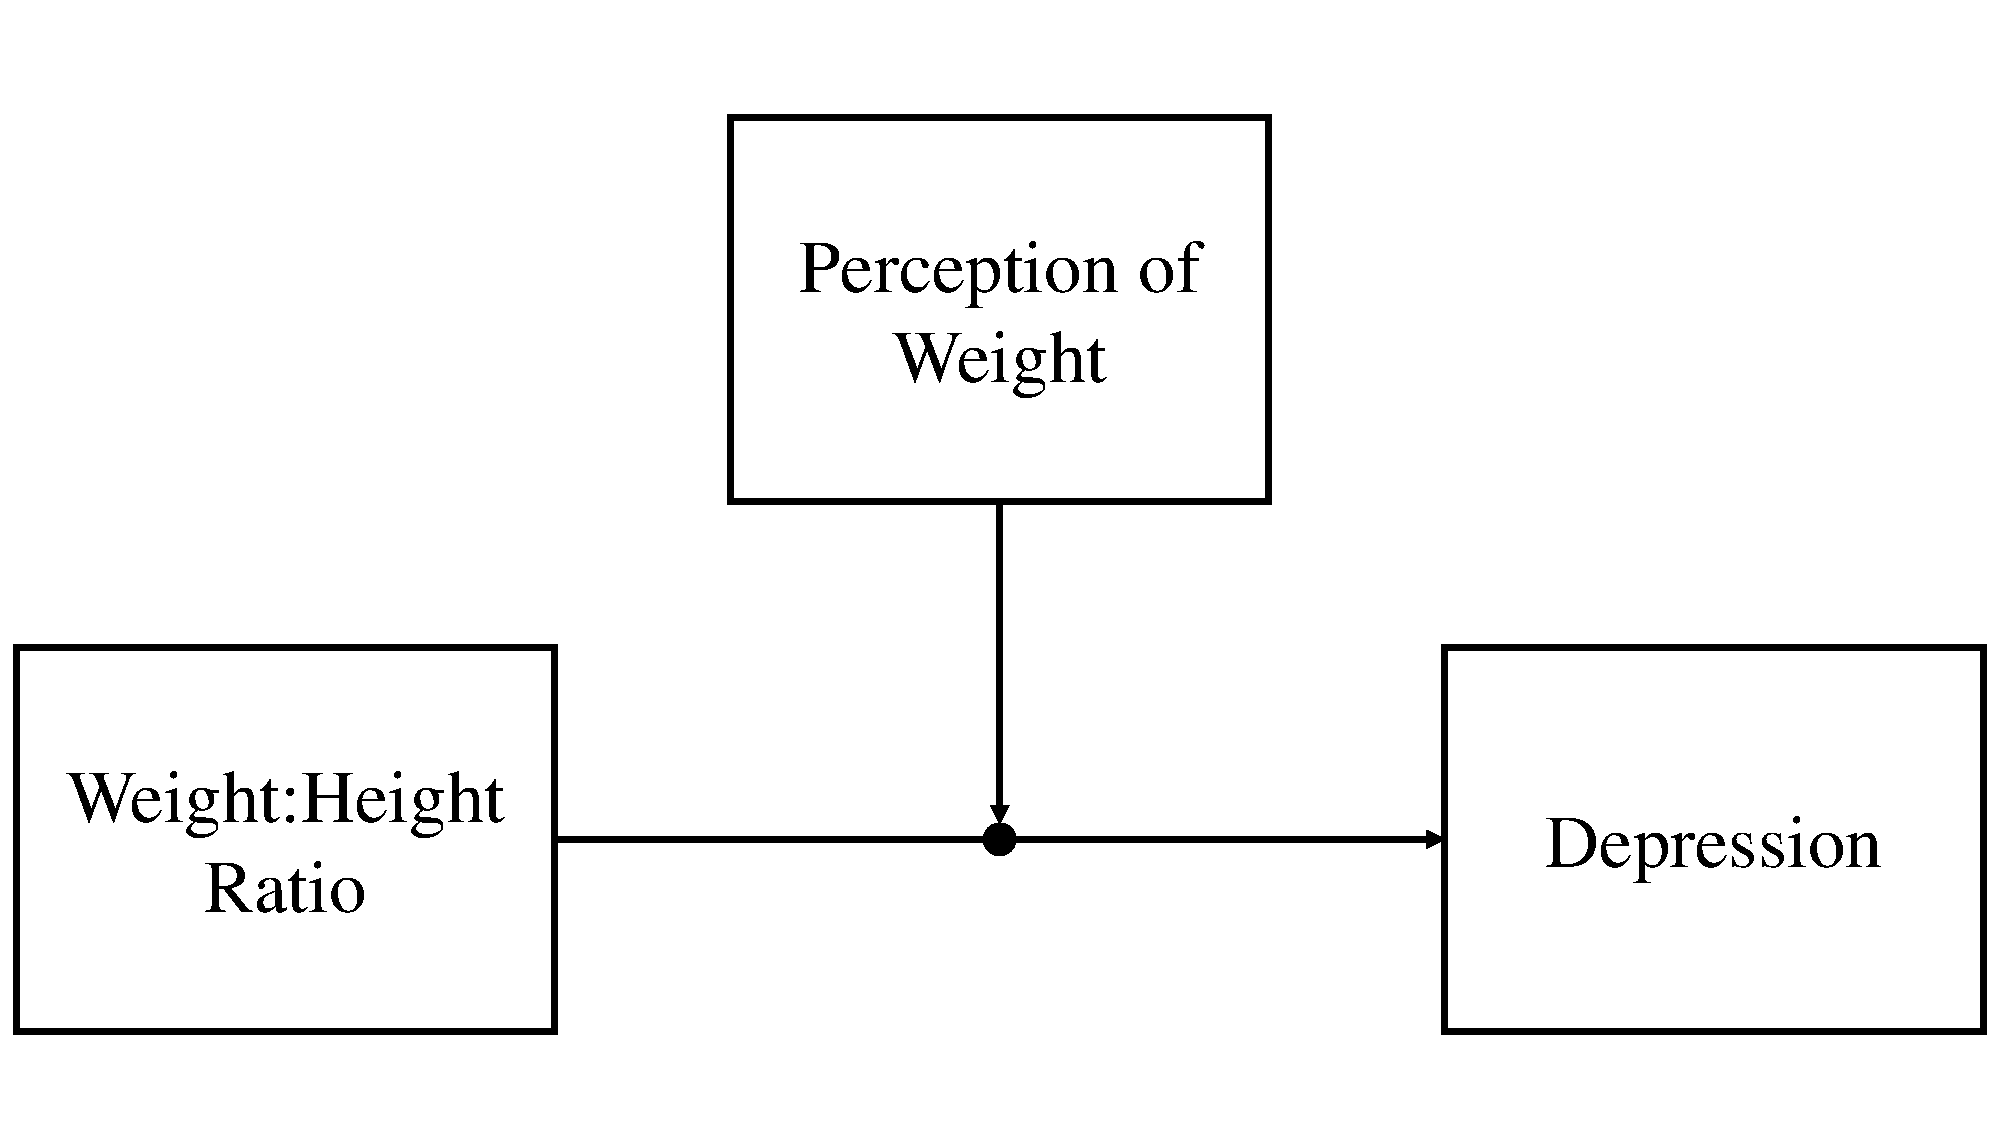
\includegraphics[width=\textwidth]{figures/modExample1.pdf}
  \end{figure}

\end{frame}



\begin{frame}{Interaction Probing}
  
  We probed the interaction with the \emph{Pick-a-point} approach.
  \va
  \begin{itemize}
    \item Choose interesting values of the moderator $Z$
      \vb
    \item Check the significance of the focal effect $X \rightarrow Y$
      at the values we choose for $Z$.
      \vb
    \item Gives us an idea of where in $Z$'s distribution the focal
      effect is/is not significant.
  \end{itemize}
  \va
  Previously, we manually calculated the all of the quantities we
  needed, including a SE for the conditional focal effect.
  \vb
  \begin{itemize}
    \item There is a simpler way: \textsc{Centering}
  \end{itemize}
  
\end{frame}



\begin{frame}{Centering}
  
  Centering transforms a variable by subtracting a constant (e.g., the
  variable's mean) from each observation of the variable
  \va
  \begin{itemize}
  \item The most familiar form of center is \emph{mean centering}
    \vb
  \item We can center on any value
    \vb
    \begin{itemize}
    \item When probing interactions, we can center $Z$ on the
      interesting values we choose during the pick-a-point approach
      \vb
    \item Running the model with $Z$ centered on specific values
      automatically provides tests of the simple slope conditional
      on those values of $Z$
    \end{itemize}
  \end{itemize}
  
\end{frame}



\begin{frame}{Probing via Centering}
  
  Say we want to do a simple slopes analysis to test the conditional
  effect of $X$ on $Y$ at three levels of $Z = \{Z_1, Z_2,
  Z_3\}$.\\ 
  \va 
  Then, all we need to do is fit the following three
  models:
  \begin{align*}
    Y = \alpha + \beta_1X + \beta_2(Z - Z_1) + \beta_3 X(Z - Z_1) + e\\
    \\
    Y = \alpha + \beta_1X + \beta_2(Z - Z_2) + \beta_3 X(Z - Z_2) + e\\
    \\
    Y = \alpha + \beta_1X + \beta_2(Z - Z_3) + \beta_3 X(Z - Z_3) + e
  \end{align*}
  The default output for $\beta_1$ provides tests of the simple
  slopes.
  
\end{frame}



\begin{frame}[allowframebreaks]{Example}

\begin{Schunk}
\begin{Sinput}
 library(lavaan)
 dataDir <- "../data/"
 dat1 <- readRDS(paste0(dataDir, "adamsKlpsData.rds"))
 ## Specify the CFA model:
 mod1.1 <- "
 merit =~ meritP1 + meritP2 + meritP3
 policy =~ policyP1 + policyP2 + policyP3
 "
 ## Fit the CFA and check model:
 out1.1 <- cfa(mod1.1, data = dat1, std.lv = TRUE)
 ## Check model fit:
 round(fitMeasures(out1.1)[c("chisq", "df", "pvalue", "cfi", 
                             "tli", "rmsea", "srmr")], 4)
\end{Sinput}
\begin{Soutput}
  chisq      df  pvalue     cfi     tli   rmsea    srmr 
16.8695  8.0000  0.0315  0.9215  0.8529  0.1129  0.0653 
\end{Soutput}
\begin{Sinput}
 summary(out1.1)
\end{Sinput}
\begin{Soutput}
lavaan (0.5-20) converged normally after  22 iterations

  Number of observations                            87

  Estimator                                         ML
  Minimum Function Test Statistic               16.869
  Degrees of freedom                                 8
  P-value (Chi-square)                           0.031

Parameter Estimates:

  Information                                 Expected
  Standard Errors                             Standard

Latent Variables:
                   Estimate  Std.Err  Z-value  P(>|z|)
  merit =~                                            
    meritP1           0.690    0.134    5.155    0.000
    meritP2           0.968    0.142    6.830    0.000
    meritP3           0.748    0.137    5.458    0.000
  policy =~                                           
    policyP1          0.851    0.186    4.570    0.000
    policyP2          0.996    0.167    5.967    0.000
    policyP3          1.121    0.177    6.339    0.000

Covariances:
                   Estimate  Std.Err  Z-value  P(>|z|)
  merit ~~                                            
    policy           -0.336    0.131   -2.563    0.010

Variances:
                   Estimate  Std.Err  Z-value  P(>|z|)
    meritP1           0.865    0.165    5.248    0.000
    meritP2           0.445    0.201    2.211    0.027
    meritP3           0.833    0.172    4.857    0.000
    policyP1          1.836    0.324    5.671    0.000
    policyP2          0.942    0.256    3.683    0.000
    policyP3          0.857    0.297    2.882    0.004
    merit             1.000                           
    policy            1.000                           
\end{Soutput}
\end{Schunk}


\end{frame}


\begin{frame}{Compare Approaches}
  
  The manual and the centering approaches give identical answers,
  barring rounding errors with the manual approach: 
  \va
\begin{Schunk}
\begin{Sinput}
 round(fitMeasures(out1)[c("chisq", "df", "pvalue", "cfi", 
                           "tli", "rmsea", "srmr")], 3)
\end{Sinput}
\begin{Soutput}
 chisq     df pvalue    cfi    tli  rmsea   srmr 
41.021 24.000  0.017  0.987  0.981  0.038  0.026 
\end{Soutput}
\end{Schunk}


\end{frame}



\begin{frame}[allowframebreaks]{A Few Comments on Centering}
  
  You will often hear mean centering touted as absolutely necessary or
  absolutely unnecessary for moderation analysis.\\ 
  \va 
  Both sides are partially correct.\\ 
  \va 
  Two effects are usually ascribed to mean
  centering in moderation analysis: 
  \vb
  \begin{enumerate}
    \item Improved interpretation of the conditional effects 
      \vb
    \item Reduced multicollinearity between lower-order effects and
      the interaction term
  \end{enumerate}
  
  \pagebreak
  
  Mean center absolutely \emph{does} have the potential to improve
  parameter interpretations
  \vb
  \begin{itemize}
  \item When $X = 0$ or $Z = 0$ are not sensible values, centering is
    necessary for any plausible interpretation of $\beta_1$ or
    $\beta_2$.
  \end{itemize}
  \va 
  Mean centering \emph{can} remove collinearity between lower-order
  terms and the interaction term
  \vb
  \begin{itemize}
    \item \textbf{BUT}, we don't care
  \end{itemize}
  \va 
  We can get a better sense of what's going on with a synthetic
  example.
\end{frame}


\begin{frame}[allowframebreaks]{Example}
    
\begin{Schunk}
\begin{Sinput}
 mod3 <- "
 att3 ~ att2 + b2*conf2 + cp2*horn2
 att2 ~ att1 + b1*conf1 + cp1*horn1
 
 conf3 ~ conf2 + a2*horn2
 conf2 ~ conf1 + a1*horn1
 
 horn3 ~ horn2
 horn2 ~ horn1
 
 horn3 ~~ conf3 + att3
 conf3 ~~ att3
 
 horn2 ~~ conf2 + att2
 conf2 ~~ att2
 
 a1 == a2
 b1 == b2
 cp1 == cp2
 "
 out3 <- sem(mod3, data = dat1)
 summary(out3)
\end{Sinput}
\begin{Soutput}
lavaan (0.5-20) converged normally after  46 iterations

  Number of observations                           500

  Estimator                                         ML
  Minimum Function Test Statistic              294.220
  Degrees of freedom                                18
  P-value (Chi-square)                           0.000

Parameter Estimates:

  Information                                 Expected
  Standard Errors                             Standard

Regressions:
                   Estimate  Std.Err  Z-value  P(>|z|)
  att3 ~                                              
    att2              0.497    0.035   14.234    0.000
    conf2     (b2)    0.098    0.019    5.200    0.000
    horn2    (cp2)    0.083    0.072    1.157    0.247
  att2 ~                                              
    att1              0.530    0.040   13.345    0.000
    conf1     (b1)    0.098    0.019    5.200    0.000
    horn1    (cp1)    0.083    0.072    1.157    0.247
  conf3 ~                                             
    conf2             0.684    0.035   19.602    0.000
    horn2     (a2)    0.493    0.107    4.596    0.000
  conf2 ~                                             
    conf1             0.623    0.032   19.546    0.000
    horn1     (a1)    0.493    0.107    4.596    0.000
  horn3 ~                                             
    horn2             0.826    0.030   27.609    0.000
  horn2 ~                                             
    horn1             0.714    0.024   29.181    0.000

Covariances:
                   Estimate  Std.Err  Z-value  P(>|z|)
  conf3 ~~                                            
    horn3             1.016    0.155    6.556    0.000
  att3 ~~                                             
    horn3             0.322    0.093    3.483    0.000
    conf3             3.574    0.465    7.691    0.000
  conf2 ~~                                            
    horn2             0.836    0.124    6.721    0.000
  att2 ~~                                             
    horn2             0.273    0.083    3.289    0.001
    conf2             2.027    0.400    5.067    0.000

Variances:
                   Estimate  Std.Err  Z-value  P(>|z|)
    att3              6.019    0.381   15.811    0.000
    att2              6.041    0.382   15.811    0.000
    conf3            15.814    1.000   15.811    0.000
    conf2            12.570    0.795   15.811    0.000
    horn3             0.695    0.044   15.811    0.000
    horn2             0.560    0.035   15.811    0.000

Constraints:
                                               |Slack|
    a1 - (a2)                                    0.000
    b1 - (b2)                                    0.000
    cp1 - (cp2)                                  0.000
\end{Soutput}
\begin{Sinput}
 chiDiff <- fitMeasures(out3)["chisq"] -
     fitMeasures(out1)["chisq"]
 dfDiff <- fitMeasures(out3)["df"] -
     fitMeasures(out1)["df"]
 pchisq(chiDiff, dfDiff, lower = FALSE)
\end{Sinput}
\begin{Soutput}
     chisq 
0.02684148 
\end{Soutput}
\end{Schunk}


\pagebreak

\begin{Schunk}
\begin{Sinput}
 mod4 <- "
 att3 ~ att2 + b2*conf2 + cp*horn1
 att2 ~ att1 + b1*conf1
 
 conf3 ~ conf2 + a2*horn2
 conf2 ~ conf1 + a1*horn1
 
 att2 + att3 ~ income
 conf2 + conf3 ~ income 
 horn2 + horn3 ~ income
 
 horn3 ~ horn2
 horn2 ~ horn1
 
 horn3 ~~ conf3 + att3
 conf3 ~~ att3
 
 horn2 ~~ conf2 + att2
 conf2 ~~ att2
 
 ab := a1*b2
 "
 out4 <- sem(mod4, data = dat1, se = "boot", boot = nBoot)
 summary(out4)
\end{Sinput}
\begin{Soutput}
lavaan (0.5-20) converged normally after  63 iterations

  Number of observations                           500

  Estimator                                         ML
  Minimum Function Test Statistic              219.789
  Degrees of freedom                                16
  P-value (Chi-square)                           0.000

Parameter Estimates:

  Information                                 Observed
  Standard Errors                            Bootstrap
  Number of requested bootstrap draws             2000
  Number of successful bootstrap draws            2000

Regressions:
                   Estimate  Std.Err  Z-value  P(>|z|)
  att3 ~                                              
    att2              0.513    0.039   13.099    0.000
    conf2     (b2)    0.022    0.027    0.826    0.409
    horn1     (cp)   -0.119    0.084   -1.418    0.156
  att2 ~                                              
    att1              0.477    0.043   10.980    0.000
    conf1     (b1)    0.084    0.028    3.048    0.002
  conf3 ~                                             
    conf2             0.488    0.041   11.803    0.000
    horn2     (a2)    0.492    0.160    3.076    0.002
  conf2 ~                                             
    conf1             0.543    0.037   14.594    0.000
    horn1     (a1)    0.175    0.146    1.204    0.228
  att2 ~                                              
    income            0.052    0.013    4.108    0.000
  att3 ~                                              
    income            0.057    0.012    4.853    0.000
  conf2 ~                                             
    income            0.110    0.016    6.871    0.000
  conf3 ~                                             
    income            0.148    0.018    8.206    0.000
  horn2 ~                                             
    income            0.016    0.003    5.698    0.000
  horn3 ~                                             
    income            0.013    0.004    3.555    0.000
    horn2             0.780    0.033   23.921    0.000
  horn2 ~                                             
    horn1             0.654    0.026   25.525    0.000

Covariances:
                   Estimate  Std.Err  Z-value  P(>|z|)
  conf3 ~~                                            
    horn3             0.915    0.152    6.020    0.000
  att3 ~~                                             
    horn3             0.322    0.092    3.489    0.000
    conf3             2.971    0.412    7.215    0.000
  conf2 ~~                                            
    horn2             0.678    0.112    6.026    0.000
  att2 ~~                                             
    horn2             0.203    0.083    2.428    0.015
    conf2             1.601    0.382    4.194    0.000

Variances:
                   Estimate  Std.Err  Z-value  P(>|z|)
    att3              5.771    0.351   16.431    0.000
    att2              5.821    0.362   16.099    0.000
    conf3            14.066    0.828   16.988    0.000
    conf2            11.512    0.729   15.792    0.000
    horn2             0.529    0.033   16.004    0.000
    horn3             0.677    0.040   16.788    0.000

Defined Parameters:
                   Estimate  Std.Err  Z-value  P(>|z|)
    ab                0.004    0.007    0.559    0.576
\end{Soutput}
\begin{Sinput}
 parameterEstimates(out4, boot = "bca.simple")[ , -c(1 : 3)]
\end{Sinput}
\begin{Soutput}
   label     est    se      z pvalue ci.lower ci.upper
1          0.513 0.039 13.099  0.000    0.438    0.589
2     b2   0.022 0.027  0.826  0.409   -0.030    0.076
3     cp  -0.119 0.084 -1.418  0.156   -0.275    0.051
4          0.477 0.043 10.980  0.000    0.396    0.565
5     b1   0.084 0.028  3.048  0.002    0.029    0.139
6          0.488 0.041 11.803  0.000    0.410    0.569
7     a2   0.492 0.160  3.076  0.002    0.186    0.818
8          0.543 0.037 14.594  0.000    0.464    0.614
9     a1   0.175 0.146  1.204  0.228   -0.099    0.468
10         0.052 0.013  4.108  0.000    0.028    0.077
11         0.057 0.012  4.853  0.000    0.033    0.079
12         0.110 0.016  6.871  0.000    0.079    0.141
13         0.148 0.018  8.206  0.000    0.114    0.183
14         0.016 0.003  5.698  0.000    0.011    0.022
15         0.013 0.004  3.555  0.000    0.005    0.019
16         0.780 0.033 23.921  0.000    0.714    0.844
17         0.654 0.026 25.525  0.000    0.601    0.703
18         0.915 0.152  6.020  0.000    0.633    1.225
19         0.322 0.092  3.489  0.000    0.143    0.508
20         2.971 0.412  7.215  0.000    2.207    3.834
21         0.678 0.112  6.026  0.000    0.466    0.903
22         0.203 0.083  2.428  0.015    0.040    0.369
23         1.601 0.382  4.194  0.000    0.870    2.387
24         5.771 0.351 16.431  0.000    5.130    6.509
25         5.821 0.362 16.099  0.000    5.171    6.590
26        14.066 0.828 16.988  0.000   12.623   15.934
27        11.512 0.729 15.792  0.000   10.207   13.077
28         0.529 0.033 16.004  0.000    0.472    0.602
29         0.677 0.040 16.788  0.000    0.606    0.765
30         1.809 0.000     NA     NA    1.809    1.809
31         1.470 0.000     NA     NA    1.470    1.470
32         3.939 0.000     NA     NA    3.939    3.939
33         5.753 0.000     NA     NA    5.753    5.753
34         8.748 0.000     NA     NA    8.748    8.748
35         8.475 0.000     NA     NA    8.475    8.475
36        16.763 0.000     NA     NA   16.763   16.763
37        28.025 0.000     NA     NA   28.025   28.025
38        39.156 0.000     NA     NA   39.156   39.156
39       136.353 0.000     NA     NA  136.353  136.353
40    ab   0.004 0.007  0.559  0.576   -0.003    0.031
\end{Soutput}
\end{Schunk}

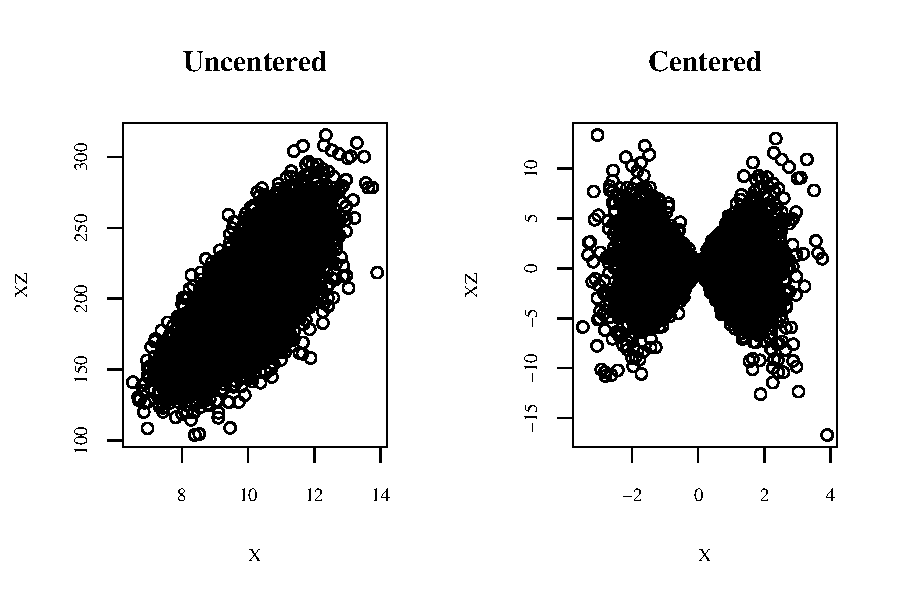
\includegraphics{sweaveFiles/-005}

\end{frame}


\begin{frame}[shrink = 10]{Example}
  
\begin{Schunk}
\begin{Sinput}
 ## Completely Standardized:
 abCS <- (sdX * ab) / sdY
 abCS
\end{Sinput}
\begin{Soutput}
[1] 0.1345859
\end{Soutput}
\begin{Sinput}
 cPrimeCS <- (sdX * cPrime) / sdY
 cPrimeCS
\end{Sinput}
\begin{Soutput}
       cp 
0.1790413 
\end{Soutput}
\begin{Sinput}
 cCS <- abCS + cPrimeCS
 cCS
\end{Sinput}
\begin{Soutput}
       cp 
0.3136272 
\end{Soutput}
\end{Schunk}


\end{frame}


\begin{frame}[allowframebreaks]{Example}
  
\begin{Schunk}
\begin{Sinput}
 mod3 <- "
 fX =~ x1 + x2 + x3
 fZ =~ z1 + z2 + z3
 fY =~ y1 + y2 + y3
 fXZ =~ x1z1R + x1z2R + x1z3R +
 x2z1R + x2z2R + x2z3R +
 x3z1R + x3z2R + x3z3R
 
 fY ~ fX + fZ + fXZ
 
 fX ~~ fZ
 fX ~~ 0*fXZ
 fZ ~~ 0*fXZ
 
 x1z1R ~~ x1z2R + x1z3R + x2z1R + x3z1R
 x1z2R ~~ x1z3R + x2z2R + x3z2R
 x1z3R ~~ x2z3R + x3z3R
 
 x2z1R ~~ x2z2R + x2z3R + x3z1R
 x2z2R ~~ x2z3R + x3z2R
 x2z3R ~~ x3z3R
 
 x3z1R ~~ x3z2R + x3z3R
 x3z2R ~~ x3z3R
 "
 out3 <- sem(mod3, data = dat2, std.lv = TRUE)
 summary(out3)
\end{Sinput}
\begin{Soutput}
lavaan (0.5-20) converged normally after  53 iterations

  Number of observations                           500

  Estimator                                         ML
  Minimum Function Test Statistic               74.899
  Degrees of freedom                               113
  P-value (Chi-square)                           0.998

Parameter Estimates:

  Information                                 Expected
  Standard Errors                             Standard

Latent Variables:
                   Estimate  Std.Err  Z-value  P(>|z|)
  fX =~                                               
    x1                0.670    0.043   15.424    0.000
    x2                0.660    0.043   15.256    0.000
    x3                0.704    0.045   15.569    0.000
  fZ =~                                               
    z1                0.738    0.048   15.342    0.000
    z2                0.734    0.048   15.156    0.000
    z3                0.718    0.046   15.602    0.000
  fY =~                                               
    y1                0.396    0.046    8.545    0.000
    y2                0.369    0.044    8.441    0.000
    y3                0.383    0.045    8.558    0.000
  fXZ =~                                              
    x1z1R             0.361    0.053    6.833    0.000
    x1z2R             0.427    0.056    7.615    0.000
    x1z3R             0.432    0.053    8.190    0.000
    x2z1R             0.558    0.056    9.914    0.000
    x2z2R             0.616    0.062   10.008    0.000
    x2z3R             0.520    0.057    9.153    0.000
    x3z1R             0.516    0.059    8.805    0.000
    x3z2R             0.626    0.063   10.007    0.000
    x3z3R             0.521    0.058    8.936    0.000

Regressions:
                   Estimate  Std.Err  Z-value  P(>|z|)
  fY ~                                                
    fX                1.658    0.239    6.930    0.000
    fZ               -0.074    0.099   -0.750    0.453
    fXZ               0.488    0.120    4.049    0.000

Covariances:
                   Estimate  Std.Err  Z-value  P(>|z|)
  fX ~~                                               
    fZ                0.232    0.058    3.987    0.000
    fXZ               0.000                           
  fZ ~~                                               
    fXZ               0.000                           
  x1z1R ~~                                            
    x1z2R             0.273    0.032    8.397    0.000
    x1z3R             0.309    0.033    9.358    0.000
    x2z1R             0.232    0.031    7.566    0.000
    x3z1R             0.235    0.032    7.376    0.000
  x1z2R ~~                                            
    x1z3R             0.231    0.032    7.243    0.000
    x2z2R             0.211    0.035    5.982    0.000
    x3z2R             0.250    0.041    6.163    0.000
  x1z3R ~~                                            
    x2z3R             0.213    0.030    7.010    0.000
    x3z3R             0.213    0.034    6.312    0.000
  x2z1R ~~                                            
    x2z2R             0.247    0.043    5.787    0.000
    x2z3R             0.252    0.040    6.368    0.000
    x3z1R             0.233    0.033    7.103    0.000
  x2z2R ~~                                            
    x2z3R             0.304    0.043    7.086    0.000
    x3z2R             0.199    0.040    5.018    0.000
  x2z3R ~~                                            
    x3z3R             0.139    0.030    4.570    0.000
  x3z1R ~~                                            
    x3z2R             0.212    0.041    5.116    0.000
    x3z3R             0.260    0.040    6.454    0.000
  x3z2R ~~                                            
    x3z3R             0.157    0.041    3.846    0.000

Variances:
                   Estimate  Std.Err  Z-value  P(>|z|)
    x1                0.511    0.042   12.093    0.000
    x2                0.514    0.042   12.221    0.000
    x3                0.548    0.046   11.977    0.000
    z1                0.523    0.052   10.142    0.000
    z2                0.546    0.052   10.444    0.000
    z3                0.461    0.048    9.704    0.000
    y1                0.495    0.043   11.398    0.000
    y2                0.542    0.044   12.334    0.000
    y3                0.444    0.040   11.179    0.000
    x1z1R             0.743    0.050   14.912    0.000
    x1z2R             0.754    0.055   13.682    0.000
    x1z3R             0.694    0.050   13.824    0.000
    x2z1R             0.641    0.057   11.332    0.000
    x2z2R             0.708    0.067   10.575    0.000
    x2z3R             0.671    0.056   12.009    0.000
    x3z1R             0.736    0.060   12.310    0.000
    x3z2R             0.724    0.070   10.277    0.000
    x3z3R             0.707    0.060   11.823    0.000
    fX                1.000                           
    fZ                1.000                           
    fY                1.000                           
    fXZ               1.000                           
\end{Soutput}
\end{Schunk}


\pagebreak

\begin{Schunk}
\begin{Sinput}
 parameterEstimates(out2.1, boot = bootType)[ , -c(1 : 3)]
\end{Sinput}
\begin{Soutput}
     label    est    se      z pvalue ci.lower ci.upper
1       b1 -0.008 0.145 -0.052  0.959   -0.286    0.275
2       b2  0.595 0.142  4.184  0.000    0.317    0.861
3       cp  0.134 0.076  1.763  0.078   -0.019    0.281
4      d21 -0.301 0.110 -2.733  0.006   -0.508   -0.076
5       a2  0.090 0.072  1.253  0.210   -0.073    0.220
6       a1 -0.266 0.061 -4.384  0.000   -0.384   -0.148
7           0.987 0.164  6.013  0.000    0.733    1.390
8           0.689 0.094  7.309  0.000    0.537    0.919
9           0.719 0.112  6.389  0.000    0.535    0.980
10          2.444 0.000     NA     NA    2.444    2.444
11     ab1  0.002 0.040  0.050  0.960   -0.080    0.081
12     ab2  0.053 0.044  1.215  0.225   -0.031    0.146
13  fullIE  0.048 0.026  1.822  0.068    0.012    0.117
14 totalIE  0.103 0.048  2.145  0.032    0.011    0.202
\end{Soutput}
\end{Schunk}


\pagebreak

\begin{Schunk}
\begin{Sinput}
 ## Possible range of a:
 aMarg <- sqrt(s2M * s2Y - sYM^2) * sqrt(s2X * s2Y - sYX^2)
 aInt <- c(
     (sYM * sYX - aMarg) / (s2X * s2Y),
     (sYM * sYX + aMarg) / (s2X * s2Y)
 )
 aInt
\end{Sinput}
\begin{Soutput}
[1] -0.4378558  0.5793099
\end{Soutput}
\begin{Sinput}
 ##
 ## Possible range of b:
 bMarg <- sqrt(s2X * s2Y - sYX^2) / sqrt(s2X * s2M - sMX^2)
 bInt <- c(-1 * bMarg, bMarg)
 bInt
\end{Sinput}
\begin{Soutput}
[1] -1.289996  1.289996
\end{Soutput}
\begin{Sinput}
 ##
 ## max(a):
 aMax <- ifelse(coef(out2)["a"] < 0,
                aInt[1],
                aInt[2])
 aMax
\end{Sinput}
\begin{Soutput}
        a 
0.5793099 
\end{Soutput}
\begin{Sinput}
 ##
 ## max(b)
 bMax <- ifelse(coef(out2)["b"] < 0,
                bInt[1],
                bInt[2])
 bMax
\end{Sinput}
\begin{Soutput}
       b 
1.289996 
\end{Soutput}
\begin{Sinput}
 ##
 ## max(ab)
 abMax <- aMax * bMax
 abMax
\end{Sinput}
\begin{Soutput}
        a 
0.7473075 
\end{Soutput}
\begin{Sinput}
 ##
 ## Kappa Squared:
 k2 <- ab / abMax
 k2
\end{Sinput}
\begin{Soutput}
        a 
0.1359491 
\end{Soutput}
\end{Schunk}


\pagebreak

\begin{Schunk}
\begin{Sinput}
 ## Three-way interaction model:
 out1.3 <- lm(agree ~ open*conc*neuro, data = dat1)
 summary(out1.3)
\end{Sinput}
\begin{Soutput}
Call:
lm(formula = agree ~ open * conc * neuro, data = dat1)

Residuals:
     Min       1Q   Median       3Q      Max 
-2.79789 -0.41779  0.09925  0.47556  2.10928 

Coefficients:
                Estimate Std. Error t value Pr(>|t|)    
(Intercept)     -0.58747    0.96633  -0.608  0.54328    
open             1.27903    0.25747   4.968 7.23e-07 ***
conc             1.20831    0.26559   4.550 5.63e-06 ***
neuro            0.73766    0.32240   2.288  0.02222 *  
open:conc       -0.29722    0.06935  -4.286 1.89e-05 ***
open:neuro      -0.21616    0.08091  -2.672  0.00760 ** 
conc:neuro      -0.25632    0.08244  -3.109  0.00190 ** 
open:conc:neuro  0.06541    0.02028   3.225  0.00128 ** 
---
Signif. codes:  0 ‘***’ 0.001 ‘**’ 0.01 ‘*’ 0.05 ‘.’ 0.1 ‘ ’ 1

Residual standard error: 0.6945 on 2544 degrees of freedom
Multiple R-squared:  0.07189,	Adjusted R-squared:  0.06933 
F-statistic: 28.15 on 7 and 2544 DF,  p-value: < 2.2e-16
\end{Soutput}
\end{Schunk}


\pagebreak

\begin{Schunk}
\begin{Sinput}
 ## Test Differences between Indirect Effects
 ## in Serial Multiple Mediator Model (Method 1):
 mod2.3 <- "
 policy ~ cp*polAffil + b1*merit + b2*sysRac
 merit ~ a1*polAffil
 sysRac ~ a2*polAffil + d21*merit
 
 ab1 := a1*b1
 ab2 := a2*b2
 fullIE := a1*d21*b2
 totalIE := ab1 + ab2 + fullIE 
 
 fullIE == ab1
 fullIE == ab2
 "
 out2.3 <- 
     sem(mod2.3, data = dat1, se = "boot", boot = nBoot)
 summary(out2.3)
\end{Sinput}
\begin{Soutput}
lavaan (0.5-20) converged normally after 213 iterations

  Number of observations                            87

  Estimator                                         ML
  Minimum Function Test Statistic                1.334
  Degrees of freedom                                 2
  P-value (Chi-square)                           0.513

Parameter Estimates:

  Information                                 Observed
  Standard Errors                            Bootstrap
  Number of requested bootstrap draws             2500
  Number of successful bootstrap draws            2500

Regressions:
                   Estimate  Std.Err  Z-value  P(>|z|)
  policy ~                                            
    polAffil  (cp)    0.108    0.084    1.281    0.200
    merit     (b1)   -0.150    0.047   -3.183    0.001
    sysRac    (b2)    0.521    0.125    4.157    0.000
  merit ~                                             
    polAffil  (a1)   -0.271    0.057   -4.750    0.000
  sysRac ~                                            
    polAffil  (a2)    0.078    0.025    3.125    0.002
    merit    (d21)   -0.287    0.075   -3.814    0.000

Variances:
                   Estimate  Std.Err  Z-value  P(>|z|)
    policy            1.001    0.171    5.854    0.000
    merit             0.719    0.114    6.330    0.000
    sysRac            0.690    0.090    7.632    0.000

Defined Parameters:
                   Estimate  Std.Err  Z-value  P(>|z|)
    ab1               0.041    0.014    2.983    0.003
    ab2               0.041    0.014    2.983    0.003
    fullIE            0.041    0.014    2.983    0.003
    totalIE           0.122    0.041    2.983    0.003

Constraints:
                                               |Slack|
    fullIE - (ab1)                               0.000
    fullIE - (ab2)                               0.000
\end{Soutput}
\begin{Sinput}
 ## Conduct a chi-squared difference test:
 chiDiff <- fitMeasures(out2.3)["chisq"] - 
     fitMeasures(out2.1)["chisq"]
 dfDiff <- fitMeasures(out2.3)["df"] - 
     fitMeasures(out2.1)["df"]
 pchisq(chiDiff, dfDiff, lower = FALSE)
\end{Sinput}
\begin{Soutput}
    chisq 
0.5131246 
\end{Soutput}
\end{Schunk}


\end{frame}



\begin{frame}{Back to Work}
  
  \textsc{Question:} Okay, so what about our example analysis? Should
  we center the predictors in this model:
  \begin{align*}
    Depress = \alpha + \beta_1Ratio + \beta_2Perception + \beta_3 Ratio \times Perception + e
  \end{align*}

  \pause
  
  \textsc{Answer:} Yes.\\\va
  
  \pause
  
  \textsc{Question Mark II:} Why?\\\va
  
  \pause 
  
  \textsc{Answer the Second:} Because a \emph{Weight:Height} ratio of zero
  is nonsensical and zero is outside the range of \emph{Perception}.
  
\end{frame}


\begin{frame}[shrink = 10]{Example}

\begin{Schunk}
\begin{Sinput}
 ## Conditional process model with b, c paths moderated:
 mod5 <- "
 agree ~ b1*open + b2*consc + cp1*extra + cp2*neuro + 
         cp3*extraXneuro + b3*openXconsc
 open ~ a*extra
 
 cpLo  := cp1 + cp3*(-0.962268)
 cpMid := cp1 + cp3*(-0.162268)
 cpHi  := cp1 + cp3*0.837732
 
 abLo := a * (b1 + b3*(-0.4045))
 abMid := a * (b1 + b3*(-0.0045))
 abHi := a * (b1 + b3*0.3955)
 "
\end{Sinput}
\end{Schunk}


\end{frame}


\begin{frame}[shrink = 10]{Example}
  
\begin{Schunk}
\begin{Sinput}
 out5 <- sem(mod5, data = dat1, se = "boot", boot = nBoot)
 summary(out5)
\end{Sinput}
\begin{Soutput}
lavaan (0.5-20) converged normally after  18 iterations

  Number of observations                          2800

  Estimator                                         ML
  Minimum Function Test Statistic              201.443
  Degrees of freedom                                 4
  P-value (Chi-square)                           0.000

Parameter Estimates:

  Information                                 Observed
  Standard Errors                            Bootstrap
  Number of requested bootstrap draws             5000
  Number of successful bootstrap draws            5000

Regressions:
                   Estimate  Std.Err  Z-value  P(>|z|)
  agree ~                                             
    open      (b1)    0.191    0.028    6.941    0.000
    consc     (b2)    0.021    0.027    0.774    0.439
    extra    (cp1)    0.349    0.027   13.030    0.000
    neuro    (cp2)   -0.102    0.012   -8.564    0.000
    extraXnr (cp3)    0.049    0.022    2.210    0.027
    opnXcnsc  (b3)   -0.074    0.044   -1.671    0.095
  open ~                                              
    extra      (a)    0.268    0.023   11.662    0.000

Variances:
                   Estimate  Std.Err  Z-value  P(>|z|)
    agree             0.471    0.014   32.521    0.000
    open              0.294    0.010   29.875    0.000

Defined Parameters:
                   Estimate  Std.Err  Z-value  P(>|z|)
    cpLo              0.302    0.036    8.459    0.000
    cpMid             0.341    0.027   12.473    0.000
    cpHi              0.390    0.031   12.502    0.000
    abLo              0.059    0.011    5.320    0.000
    abMid             0.051    0.009    5.778    0.000
    abHi              0.043    0.009    4.788    0.000
\end{Soutput}
\end{Schunk}


\end{frame}



\begin{frame}{Alternative Probing Strategies}
  
  The pick-a-point approach is nice due to its simplicity and ease of
  interpretation, but the points we choose are totally arbitrary.
  \vb
  \begin{itemize}
    \item We may be missing important nuances that occur in some of
      the areas of $Z$'s distribution that we \emph{did not} pick.
  \end{itemize}
  \va
  \pause
  The \emph{Johnson-Neyman} technique is an alternative approach that
  removes the arbitrary choices necessary for pick-a-point.
  \vb
  \begin{itemize}
    \item Johnson-Neyman finds the \emph{region of significance}
      wherein the conditional effect of $X$ on $Y$ is statistically
      significant
      \vb
    \item Inverts the pick-a-point approach to find what cut-points on
      the moderator correspond to a critical $t$ value for the
      conditional $\beta_1$.
  \end{itemize}

\end{frame}


\begin{frame}{Johnson-Neyman Technique}
  
  With pick-a-point, we:
  \vb
  \begin{enumerate}
    \item Choose conditional values of $Z$, say $Z_1$
      \vb
    \item Calculate the simple slope $SS_1$ and standard error
      $SE_{SS1}$ associated with $Z_1$
      \vb
    \item Test $SS_1$ for significance via a simple Wald-type test:
      \begin{align}
        t = \frac{SS_1}{SE_{SS1}} \label{waldEq}
      \end{align}
  \end{enumerate}

\end{frame}


\begin{frame}{Johnson-Neyman Technique}
  
  With Johnson-Neyman, we:
  \vb
  \begin{enumerate}
  \item Choose an $\alpha$ level for our test and the corresponding
    critical value of $t$, say $t_{crit} = 1.96$ to give $\alpha =
    0.05$ in large samples.
    \vb
  \item Re-arrange Equation \ref{waldEq} into the following quadratic
    form:
    \begin{align}
      t_{crit}^2 SE_{SS}^2 - SS^2 = 0 \label{quadEq}
    \end{align}
    \vc
  \item Solve Equation \ref{quadEq} to find the two values of $Z$ that
    produce critical $t$ statistics for the conditional focal effect.
  \end{enumerate}
  
\end{frame}


\begin{frame}{Johnson-Neyman Technique}
  
  The roots produced by the Johnson-Neyman technique delineate the
  \emph{region of significance}.  
  \vb
  \begin{itemize}
  \item The conditional effect of $X$ on $Y$ is either significant
    everywhere between these two points or everywhere outside of these
    two points.  
    \vb
  \item If only one of the points falls within the observed range of
    $Z$, ignore the other point 
    \vc
    \begin{itemize}
    \item The region of significant is either everywhere above or
      below the legal root
    \end{itemize}
    \vb
  \item If neither of the roots fall within the observed range of $Z$
    then, either: 
    \vc
    \begin{enumerate}
    \item The focal effect is significant across the entire range of
      $Z$, or 
      \vc
    \item The focal effect is not significant anywhere within the
      range of $Z$
    \end{enumerate}
  \end{itemize}
  
\end{frame}


\begin{frame}{Perspectives on Simple Slopes}
  
  Recall the formula for a simple slope:
  \begin{align*}
    SS = \beta_1 + \beta_3Z
  \end{align*}
  \vc From a graphical perspective, we can think about $SS$ in, at
  least, two different ways:
  \vb
  \begin{enumerate}
  \item As a weight for $X$ that we can use to get plots of the
    conditional effect of $X$ on $Y$ at different levels of $Z$.
    \vb
  \item We can also consider how $SS$, itself, smoothly changes as a
    function of $Z$.  
  \end{enumerate}
  \va
  The latter perspective embodies the spirit of the Johnson-Neyman
  technique.
  
\end{frame}


\begin{frame}{Confidence Bands}
  
  A natural quantity to consider is a confidence interval for $SS$:
  \begin{align*}
    CI_{SS} = SS \pm t_{crit} \cdot SE_{SS}
  \end{align*}
  \vc 
  Last time, we computed a few such intervals for the interesting
  values of $Z$ we chose for the pick-a-point analysis.\\ 
  \va 
  When doing Johnson-Neyman, we can considering the values of $CI_{SS}$
  for the entire range of $Z$.  
  \vb
  \begin{itemize}
  \item These CI values define the \emph{confidence bands} of SS and
    show, for any value of $Z$, the corresponding CI for $SS$
    \vb
    \begin{itemize}
    \item As a result, we can immediately check any value of $Z$ for
      a significant simple slope
    \end{itemize}
  \end{itemize}
  
\end{frame}

  
\begin{frame}[allowframebreaks]{Example}
  
  Implementing the Johnson-Neyman technique by hand is a pain, but we
  can easily do so by using the \textbf{rockchalk} package in
  \textsf{R}\\ 
  \va
  
\begin{Schunk}
\begin{Sinput}
 ## Hybrid Multiple Mediator Model:
 mod4.1 <- "
 policy ~ b1*merit + b21*sysRac + b22*revDisc + cp*polAffil
 sysRac ~ d211*merit + a21*polAffil
 revDisc ~ d221*merit + a22*polAffil
 merit ~ a1*polAffil
 
 sysRac ~~ revDisc
 
 ab1 := a1*b1
 ab21 := a21*b21
 ab22 := a22*b22
 
 fullIE21 := a1*d211*b21
 fullIE22 := a1*d221*b22
 
 totalIE := ab1 + ab21 + ab22 + fullIE21 + fullIE22
 "
 out4.1 <- 
     sem(mod4.1, data = dat1, se = "boot", boot = nBoot)
 summary(out4.1)
\end{Sinput}
\begin{Soutput}
lavaan (0.5-20) converged normally after  22 iterations

  Number of observations                            87

  Estimator                                         ML
  Minimum Function Test Statistic                0.000
  Degrees of freedom                                 0
  Minimum Function Value               0.0000000000000

Parameter Estimates:

  Information                                 Observed
  Standard Errors                            Bootstrap
  Number of requested bootstrap draws             2500
  Number of successful bootstrap draws            2499

Regressions:
                   Estimate  Std.Err  Z-value  P(>|z|)
  policy ~                                            
    merit     (b1)    0.005    0.142    0.035    0.972
    sysRac   (b21)    0.589    0.150    3.924    0.000
    revDisc  (b22)   -0.026    0.080   -0.328    0.743
    polAffl   (cp)    0.130    0.080    1.627    0.104
  sysRac ~                                            
    merit   (d211)   -0.301    0.111   -2.721    0.006
    polAffl  (a21)    0.090    0.070    1.282    0.200
  revDisc ~                                           
    merit   (d221)    0.532    0.192    2.777    0.005
    polAffl  (a22)   -0.167    0.138   -1.214    0.225
  merit ~                                             
    polAffl   (a1)   -0.266    0.061   -4.337    0.000

Covariances:
                   Estimate  Std.Err  Z-value  P(>|z|)
  sysRac ~~                                           
    revDisc          -0.135    0.157   -0.859    0.390

Variances:
                   Estimate  Std.Err  Z-value  P(>|z|)
    policy            0.985    0.162    6.098    0.000
    sysRac            0.689    0.092    7.463    0.000
    revDisc           2.388    0.303    7.881    0.000
    merit             0.719    0.113    6.378    0.000

Defined Parameters:
                   Estimate  Std.Err  Z-value  P(>|z|)
    ab1              -0.001    0.039   -0.034    0.973
    ab21              0.053    0.043    1.247    0.212
    ab22              0.004    0.018    0.251    0.801
    fullIE21          0.047    0.025    1.871    0.061
    fullIE22          0.004    0.014    0.276    0.783
    totalIE           0.107    0.052    2.047    0.041
\end{Soutput}
\end{Schunk}

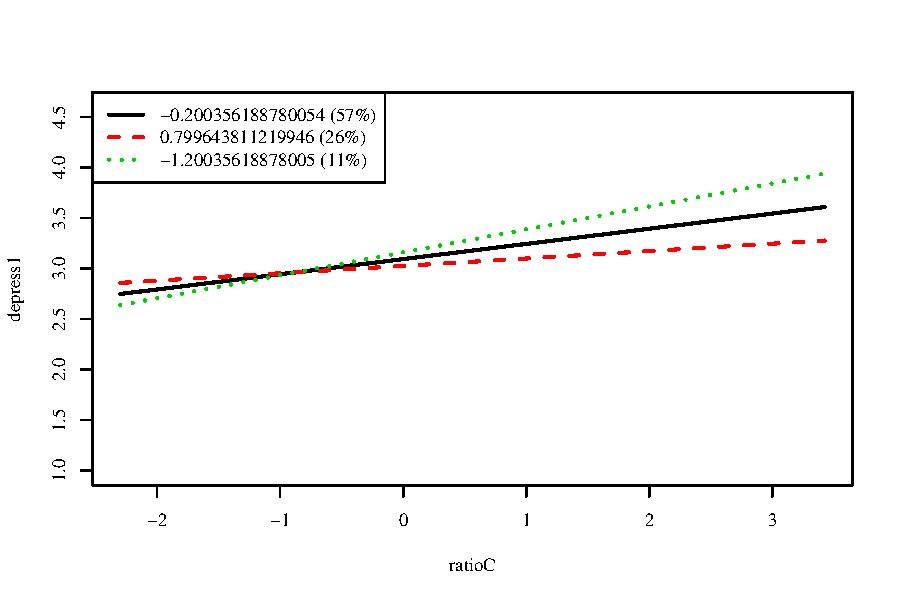
\includegraphics{sweaveFiles/-014}
\pagebreak

We can see the significance boundaries by extracting the roots from
'testOut'
\begin{Schunk}
\begin{Sinput}
 parameterEstimates(out4.1, boot = bootType)[ , -c(1 : 3)]
\end{Sinput}
\begin{Soutput}
      label    est    se      z pvalue ci.lower ci.upper
1        b1  0.005 0.142  0.035  0.972   -0.266    0.285
2       b21  0.589 0.150  3.924  0.000    0.301    0.891
3       b22 -0.026 0.080 -0.328  0.743   -0.186    0.129
4        cp  0.130 0.080  1.627  0.104   -0.029    0.283
5      d211 -0.301 0.111 -2.721  0.006   -0.520   -0.085
6       a21  0.090 0.070  1.282  0.200   -0.045    0.222
7      d221  0.532 0.192  2.777  0.005    0.137    0.899
8       a22 -0.167 0.138 -1.214  0.225   -0.447    0.099
9        a1 -0.266 0.061 -4.337  0.000   -0.396   -0.153
10          -0.135 0.157 -0.859  0.390   -0.459    0.165
11           0.985 0.162  6.098  0.000    0.750    1.477
12           0.689 0.092  7.463  0.000    0.538    0.904
13           2.388 0.303  7.881  0.000    1.894    3.158
14           0.719 0.113  6.378  0.000    0.535    1.003
15           2.444 0.000     NA     NA    2.444    2.444
16      ab1 -0.001 0.039 -0.034  0.973   -0.081    0.074
17     ab21  0.053 0.043  1.247  0.212   -0.019    0.151
18     ab22  0.004 0.018  0.251  0.801   -0.018    0.064
19 fullIE21  0.047 0.025  1.871  0.061    0.013    0.123
20 fullIE22  0.004 0.014  0.276  0.783   -0.015    0.042
21  totalIE  0.107 0.052  2.047  0.041    0.005    0.218
\end{Soutput}
\end{Schunk}

\va
We can plot the result:
\begin{Schunk}
\begin{Sinput}
 ## Use semTools to orthogonalize:
 dat2.2 <- indProd(data = dat1,
                   var1 = c("x1", "x2", "x3"),
                   var2 = c("z1", "z2", "z3"),
                   match = FALSE,
                   residualC = TRUE)
 sum(dat2 - dat2.2)
\end{Sinput}
\begin{Soutput}
[1] -9.790839e-14
\end{Soutput}
\begin{Sinput}
 ##
 ## Use semTools to double mean center:
 dat3.2 <- indProd(data = dat1,
                   var1 = c("x1", "x2", "x3"),
                   var2 = c("z1", "z2", "z3"),
                   match = FALSE,
                   doubleMC = TRUE)
 sum(dat3[ , -c(1 : 9)] - dat3.2[ , -c(1 : 9)])
\end{Sinput}
\begin{Soutput}
[1] 0
\end{Soutput}
\end{Schunk}

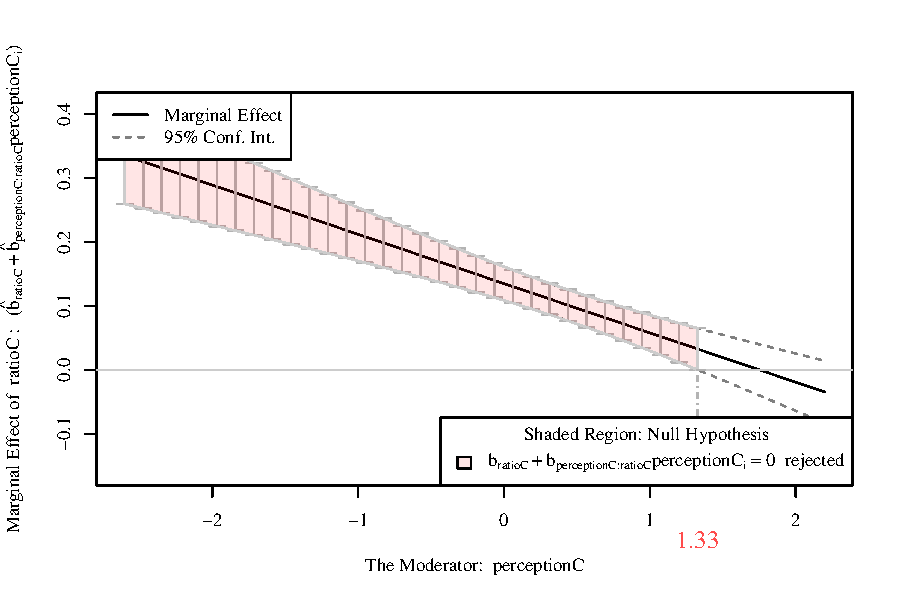
\includegraphics{sweaveFiles/-016}

\end{frame}


\end{document}
